\documentclass[12pt]{article}

\usepackage{float}
\usepackage{color}
\usepackage{caption}
\usepackage[margin=1in]{geometry}
\usepackage{amsmath}
\usepackage{xspace}
\usepackage{setspace}
\usepackage{lineno}
\usepackage{graphicx}
\usepackage{subfigure}
\begin{document}
\doublespacing
\linenumbers

\newcommand{\LLik}{\ensuremath{\text{\emph{L}}}\xspace}
\newcommand{\selac}{\emph{SelAC}\xspace}
\newcommand{\phydms}{\emph{phydms}\xspace}


\newcommand{\beginsupplement}{%
  %%% commands for getting SM pages and figures labeled with S
  %% different than with other .cls
  \setcounter{section}{19} %appendix environment set in .cls file.  Set this to 19 to get an 'S' for figures
  \setcounter{page}{1}
  \renewcommand{\thepage}{S\arabic{page}} %this works

  \setcounter{table}{0}
  \renewcommand{\thetable}{S\arabic{table}}%
  \setcounter{figure}{0}
  \renewcommand{\thefigure}{S\arabic{figure}}%
}


\noindent RH: LANDERER ET AL.--- Estimating genetic load
% put in your own RH (running head)
% for POVs the RH is always POINT OF VIEW
\bigskip
\medskip
\begin{center}

% Insert your title:
\noindent{\Large \bf Phylogenetic model of stabilizing selection is more informative about site specific selection than extrapolation from laboratory estimates.}
\bigskip

\noindent{C\textsc{EDRIC} ~{L\textsc{ANDERER}}$^{1,2,*}$,
B\textsc{RIAN} C.~ {O\textsc{MEARA}}$^{1,2}$,
\textsc{AND}
M\textsc{ICHAEL} A.~{G\textsc{ILCHRIST}}$^{1,2}$}

\end{center}

\vfill

{\small
\noindent$^{1}$Department of Ecology \& Evolutionary Biology, University of Tennessee, Knoxville, TN 37996-1610\\
\noindent$^{2}$National Institute for Mathematical and Biological Synthesis, Knoxville, TN 37996-3410\\
\noindent$^{*}$Corresponding author. E-mail:~cedric.landerer@gmail.com
}

\vfill
\centerline{Version dated: \today}
\vfill
\newpage




\section*{Introduction}
\begin{itemize}

	\item Incorporating selection into phylogenetic frameworks is already a long lasting endeavor.
	\begin{itemize}
		\item Phylogenetic inference of sequence relationship was long focused on rates of substitutions.
		\item Focus has shifted towards site specific equilibrium frequencies (HB98, Bloom2014, ...) in the last 20 years.
		\item Such models however, tend to be unfeasible as they are very parameter rich.
		\item The type of selection on a protein is not always clear, or differs between proteins phylogenetic models also have to make generalizing assumptions.
		\item Incorporating selection from experimental sources therefore seems like an attractive option.
		\item Incorporating empirical fitness has some important features.
		\begin{itemize}
			\item It allows for site specific amino acid preferences, acknowledging the heterogeneity of selection along the protein sequence.
			\item It greatly reduces the number of parameters that have to be estimated from the data.
			\item It allows for the fitting more complex models
		\end{itemize}
		\item However, the incorporation of empirical fitness also has some important short comings.
		\begin{itemize}
			\item Loss of generality.
			\item DMS experiments are limited to proteins and organisms that can be manipulated under laboratory conditions.
			\item But even in the case of TEM, the applied selection pressure is limited to the defense against a specific antibiotic.
			\item TEM, however, has evolved to compete against conspecifics and other microbes using secreted metabolites to gain an advantage.
			\item Furthermore, DMS relies on a library of mutants and therefore on a heterogeneous population with competing genotypes.
			\item Therefore, it is important to ask how adequate such experiments reflect natural evolution. 
		\end{itemize}
	\end{itemize}
	\item In this study we will assess how adequate DMS inference of site specific selection on amino acids, using TEM and provide an alternative, more generally applicable solution.
	\begin{itemize}
		\item Simulations using DMS inferred site specific selection on amino acids show that observed TEM variants are unexpected; revealing the inadequacy of DMS.
		\item Models fits achieved by the incorporation of DMS experiments can be improved upon using a hierarchical phylogenetic framework of stabilizing selection: SelAC.
		\item Extrapolating site specific selection on amino acids between sequences (TEM and SHV) with related function can be inadequate.
	\end{itemize}
\end{itemize}

\section*{Results}
\subsection*{Site Specific Selection on Amino Acids Improves Model Fit}
We compared the models \phydms and \selac, models of stabilizing site specific amino acid selection, to 281 other codon and nucleotide models by fitting them to 49 sequences of the $\beta$-lactamase TEM.
Models with site specific selection on amino acids improved model fits by 917 to 1483 AICc units over codon or nucleotide models without site specific selection (Table \ref{tab:AIC}).
In addition, \selac does outperform \phydms by 560 to  566 AICc units.

\selac utilizes a hierarchical model framework and estimates 263 site specific parameters, $\sim5\%$ of the 4997 parameters necessary to fully describe the site specific selection on amino acids.
In contrast, \phydms does not infer any site specific parameters, but utilizes site specific selection on amino acids estimated from deep mutation scanning experiments.
Incorporating site specific selection on amino acids estimated from deep mutation scanning experiments into \selac (\selac+DMS) yields similar a AICc value to \selac without that information.
This is solely due to a decrease in the number of parameters estimated, as the \LLik decreases from $-1498$ to $-1768$ (Table \ref{tab:AIC}).

\begin{table}
  \centering
  \begin{tabular}{lrrrrrr}
    Model		& \LLik &$n$ & AIC & $\Delta$AIC & AICc & $\Delta$AICc\\ \hline 
    \selac		& -1498 & 374& 3744&  0 	& 3766  & 6 \\
    \selac+DMS 	& -1768 & 111& 3758& 14	& 3760  & 0\\
    \phydms 		& -2060 & 105& 4331& 586& 4326 & 566\\
    SYM+R2 		& -2230 & 102& 4663& 919& 4694 & 934 \\
  \end{tabular}
  \caption{\LLik, number of model parameters $n$, AIC, and $\Delta$AIC., Full table has 231 models}
  \label{tab:AIC}
\end{table}


\subsection*{Laboratory inferences of selection are inconsistent with observed sequences.}
Improved model fits with phydms are deceiving.
The site specific selection inferred by the deep mutation scanning experiment is inconsistent with the observed TEM sequences.
We find that the sequence of selectively favored amino acids has only 49 \% sequence similarity with the observed consensus sequence (Figure \ref{fig:sim_seqs_cons}).
This is in contrast to the 99 \% of sequence similarity with the sequence of selectively favored amino acids estimated by \selac.

\begin{figure}[H]
     \centering
	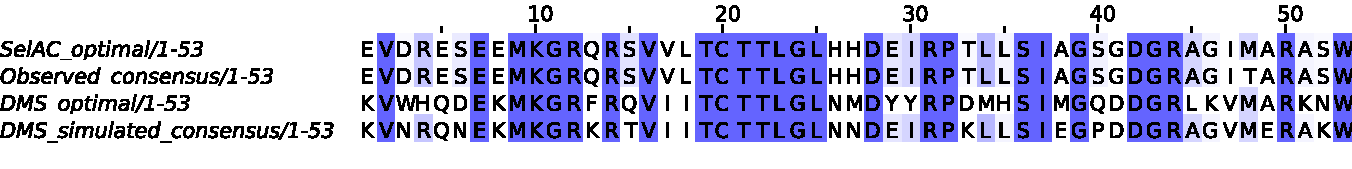
\includegraphics[width=\textwidth]{img/seq_simil_short.pdf}
	\caption{Every 5th residue. DMS and simulation based on DMS do not reflect natural sequences}
	\label{fig:sim_seqs_cons}
\end{figure}

Simulations of codon sequences under the experimentally inferred site specific selection for amino acids reveals that we would not expect to see the observed TEM sequences.
We simulated under a wide range of effective population sizes $N_e$, and find that the experimentally inferred site specific selection is very strong.
Only when $N_e$ is on the order of $10^0$ drift is overpowering the efficacy of selection.
With realistic values for $N_e$, we expect that the observed sequences show sequence similarity of $\sim 70 \%$ with the sequence of selectively favored amino acids inferred by the deep mutation scanning experiment (Figure \ref{fig:dms_sim}a).
Similarly, we expect that the substitutional load of the observed sequences should be half of the observed substitutional load (Figure \ref{fig:dms_sim}b).

\begin{figure}[h]
    \centering
    \begin{subfigure}
        \centering
        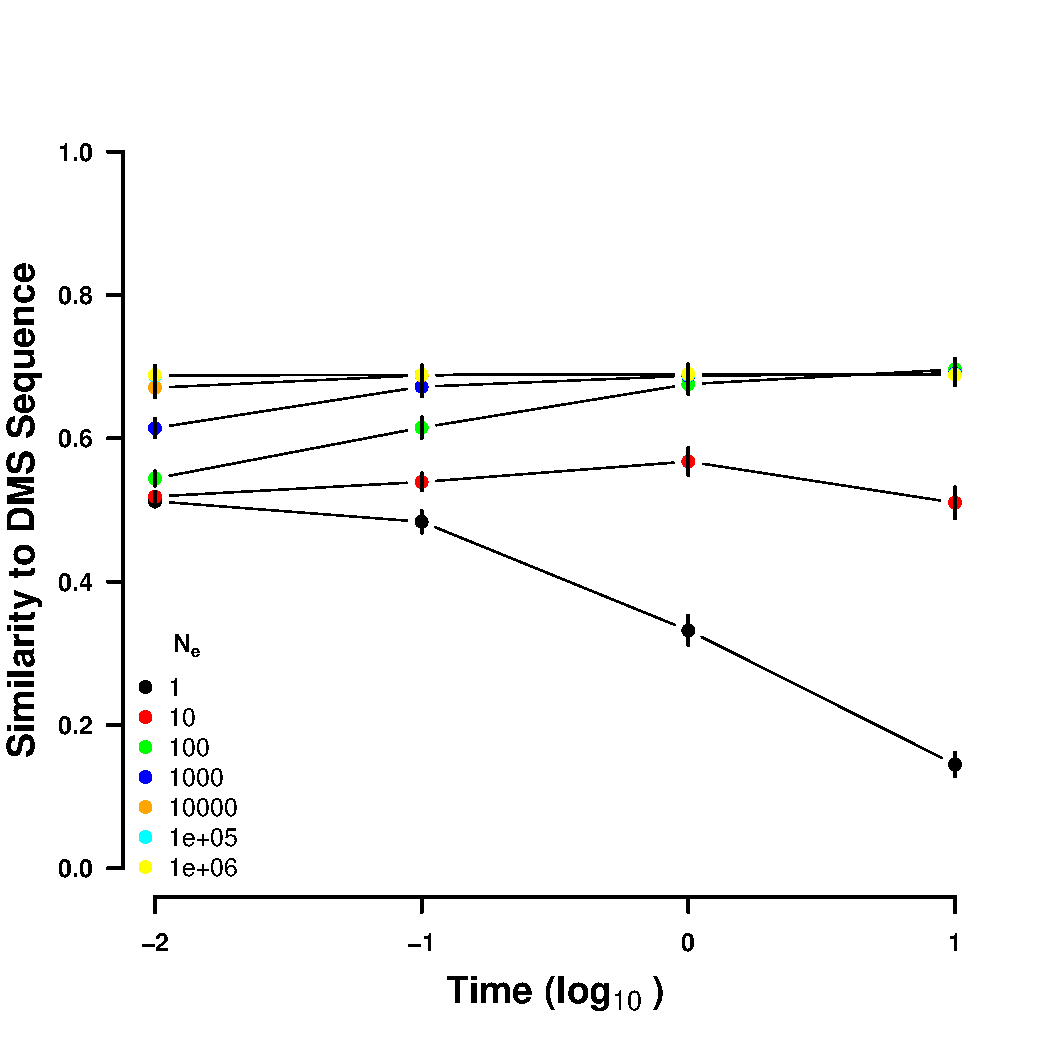
\includegraphics[width=.45\textwidth]{img/simulated_dist_time.pdf}
    \end{subfigure}
    \begin{subfigure}
        \centering
        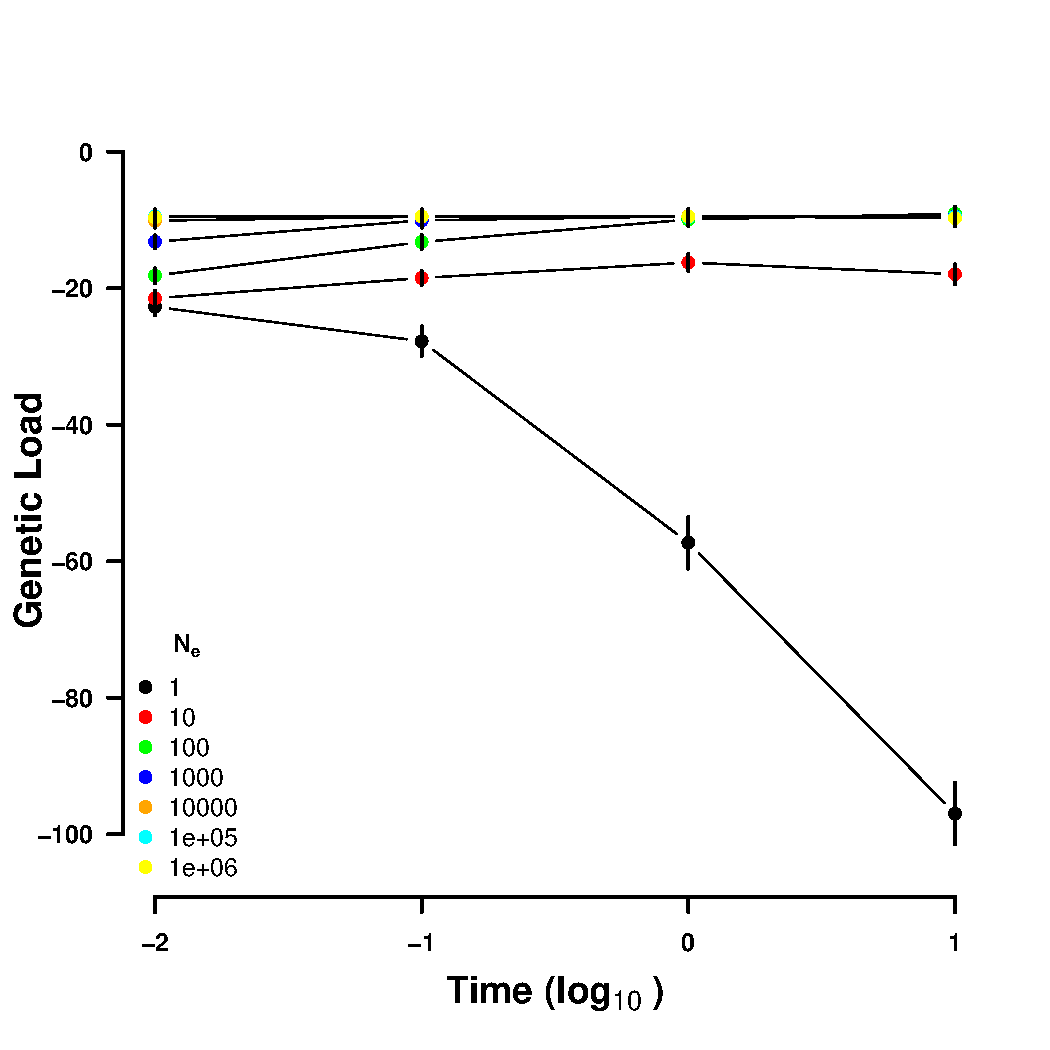
\includegraphics[width=.45\textwidth]{img/simulated_gl_time.pdf}
    \end{subfigure}
    \caption{Sequences simulated under various values of $N_e$ and for various times (expected sustitutions per site). TODO: Add starting point and observed values.}
    \label{fig:dms_sim}
\end{figure}

\subsection*{\selac Model Adequacy}
\selac better explains the observed TEM sequences.
Simulations of codon sequences under the \selac inferred site specific selection for amino acids shows high consistency with the observed TEM sequences.

\subsection*{Site specific estimates of Selection on Amino Acids}
We find that the whole sequence is under string selection and near the optimum with a small genetic load.
We find stronger selection and a higher sustitutional load in beta sheets than in helices and unstructured regions (Table \ref{tab:selection}).

\begin{table}
  \centering
  \begin{tabular}{lrrrr}
    Secondary Structure	& Mean G & SE G & Mean Subst. Load & SE Subst. Load \\ \hline 
    Helix		& 206.1 & 12.4 & -0.003 & 0.0007 \\
    Beta Sheet 		& 238.6 & 15.8 & -0.011 & 0.0094 \\
    Unstructured	& 224.8 & 11.4 & -0.006 & 0.0023 \\
    Active Sites	& 300   & 0    & 0      & 0      \\
  \end{tabular}
  \caption{\LLik, number of model parameters $n$, AIC, and $\Delta$AIC., Full table has 231 models}
  \label{tab:selection}
\end{table}

\begin{figure}[H]
     \centering
	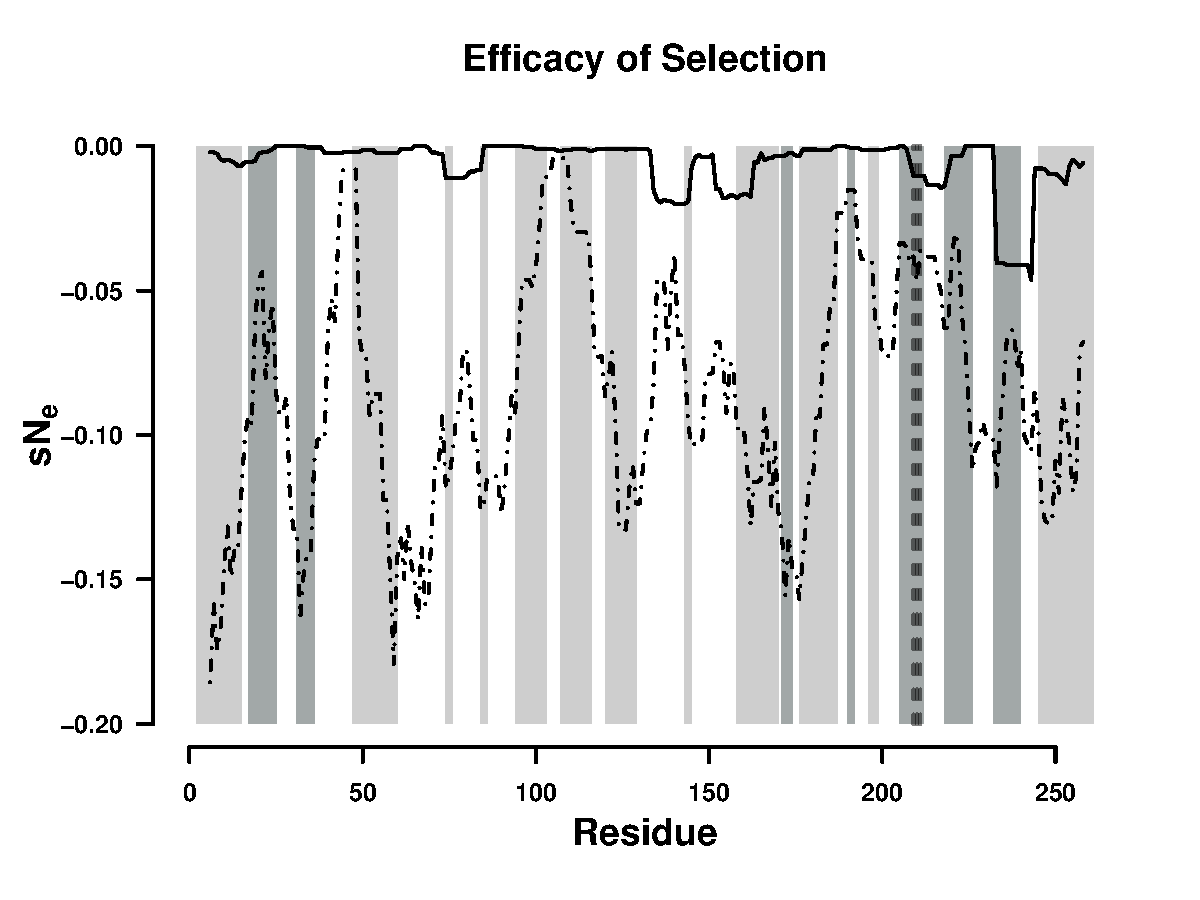
\includegraphics[width=\textwidth]{img/sNe_slide_TEM2016}
	\caption{TEM, bars are different seconday structure elements. Dashed dotted line is DMS, solid is SelAC sNe, all lines are means of all sequences, sliding window of 10 sites. vertical lines are active/binding sites.,}
	\label{fig:tem2016_sse}
\end{figure}


\begin{itemize}
	\item Site Specific Selection on Amino Acids Improves Model Fit
	\begin{itemize}
		\item phyDMS improved model fit to 49 TEM sequences by 917 AICc units
		\item Number of parameters estimated from data comparable to GY94 and others despite complex description of fitness landscape because of experimental estimates.
		\item Model selection shows that SelAC outperforms phydms (Table \ref{tab:AIC}).
	\end{itemize}

  
	\item Lab inferences of selection (DMS) are inconsistent with observed sequences.
	\begin{itemize}
 		\item The inferred fitness landscape is inconsistent with observed sequences.
		\begin{itemize}
			\item The optimal amino acid sequence inferred by DMS only shows $49 \%$ sequence similarity with the observed sequences (Figure \ref{fig:sim_seqs_cons}).
		\end{itemize}
		\item Observed sequences unlikely under the lab inferred fitness landscape (Figure \ref{fig:dms_sim}a,b).
		\begin{itemize}
			\item We would expect about half of the observed fitness burden.
			\item Sequence similarity is expected to be about $\sim 70 \%$.
		\end{itemize}
	\end{itemize}

	\item \selac Model Adequacy.
	\begin{itemize}
		\item Model adequacy assessed by sequence similarity shows that SelAC better represents the observed sequences.
	\end{itemize}

	\item Application of SelAC to TEM.
	\begin{itemize}
		\item Site specific estimates of aa fitness (Figure \ref{fig:tem2016_sse}).
		\begin{itemize}
			\item Fitness burden based on SSE.
			\item Fitness burden at binding sites
			\item Most sites show the estimated optimal amino acid.
			\item We find that selection against used amino acids is clustered and locally confined.
			\item Role of secondary structures?
		\end{itemize}
		\item Application of SelAC to TEM and comparison to TEM
		\begin{itemize}
			\item Site specific G terms for TEM and SHV are only weakly correlated ($\rho = 0.17$), despite similar $\alpha_G$ (Figure \ref{fig:tem_shv_param_comp}a).
			\item Greatest difference is observed in the physicochemical properties, specifically $\alpha$ (which PC is that?) (Figure \ref{fig:tem_shv_param_comp}b).
		\end{itemize}
	\end{itemize}
\end{itemize}

\section*{Discussion}

\begin{itemize}
	\item We evaluated how well experimental selection estimates from DMS experiments explain natural sequence evolution and compared it to a novel phylogenetic framework, SelAC.
	\begin{itemize}
		\item Previous work has shown that DMS selection estimates can improve model fit over classical approaches like GY94 and our work confirms this.
		\item Model selection favored the SelAC model fit and the corresponding fitness estimates over the DMS estimates using both, SelAC and phyDMS (Table \ref{tab:AIC}).
	\end{itemize}

	\item Adequacy of the DMS selection has previously not been assessed.
	\begin{itemize}	
		\item The amino acid with the cumulative highest fitness experimentally estimated with DMS only has $49 \%$ concordance with the observed alignment.
		\item In contrast, the SelAC estimate has $99 \%$ concordance (Figure \ref{fig:sim_seqs_cons}). 
		\item Estimates of selection coefficients do not represent evolution.
 		\begin{itemize}
			\item Due to artificial selection environment; Heterogeneous population, very large $s$. 
			\item Only one antibiotic used, maybe a mixture of antibiotics would better reflect natural evolution.
			\item Lack of repeatability between labs introduces further problems (Firnberg et al 2014 vs. Stifler et al. 2016).
		\end{itemize}
	\end{itemize}

	\item Assuming that the DMS selection inference adequately reflects natural evolution, the observed TEM sequences are either mal-adapted or where unable to reach a fitness peak.
	\begin{itemize}
		\item \textit{E. coli} has a large effective population size, estimates are on the order of $10^8$ to $10^9$ (Ochman and Wilson 1987, Hartl et al 1994).
		\item The large $N_e$ would allow \textit{E. coli} to effectively "explore" the sequence space, thus suggesting that the TEM sequences are mal-adapted according to the DMS estimates.
		\item Our simulations of sequence evolution with various $N_e$ values and the DMS fitness values in contrast show that we would expect higher adaptation even with much smaller $N_e$ (Figure \ref{fig:dms_sim}).
	\end{itemize}

	\item Estimates of selection coefficients do not represent evolution.
 	\begin{itemize}
		\item Due to artificial selection environment; Heterogeneous population, very large $s$. 
		\item Only one antibiotic used, maybe a mixture of antibiotics would better reflect natural evolution.
		\item Lack of repeatability between labs introduces further problems (Firnberg et al 2014 vs. Stifler et al. 2016).
	\end{itemize}

	\item DMS estimates of the observed TEM variants predict them to be mal-adapted while SelAC predicts most TEM variants to be well adapted.
	\begin{itemize}
		\item Given \textit{E. coli}'s large effective population size, the efficacy of selection should be very large.
		\item We therefore expect the observed sequence variants to be at the selection-mutation-drift barrier, which in turn can expected to be near the optimum.
		\item We find the majority of sequences near the optimum, therefore the SelAC estimates are consistent with theoretical population genetics results.
		\item In contrast, finding strong selection against the observed TEM variants indicates that DMS is not consistent with theoretical population genetics expectations.
		\item This is consistent when thinking about that DMS only reflects the selection on the TEM sequence with regards to one antibiotic, which seems appropriate to model selection in modern hospital environments but not when the interest lies in the natural evolution of TEM.
	\end{itemize}

	\item We find that SelAC produces similar selection against the observed TEM variants  if we assume the fitness peaks (optimal AA) that are estimated by DMS.
	\begin{itemize}
		\item This shows that DMS and SelAC can provide consistent estimates of selection against amino acids.
		\item SelAC has the advantage that it can be applied to any protein coding sequence alignment.
		\item This removes the need for extrapolation e.g. from TEM to SHV.
	\end{itemize}

	\item SelAC has the advantage that it can be applied to any protein coding sequence alignment.
	\begin{itemize}
		\item This removes the need for extrapolation e.g. from TEM to SHV.
	\end{itemize}

	\item Difference in selection parameters between TEM and SHV indicate that extrapolation is not a good idea.
	\begin{itemize}
		\item The difference in the site specific strength of selection shows that TEM and SHV are facing different selection pressures.
		\item this is also highlighted by the differences in physicochemical weightings between the two proteins.
	\end{itemize}

	\item SelAC outperforms DMS, but is not without flaws itself
	\begin{itemize}
		\item Like DMS and most phylogenetic models, SelAC assumes site independence.
		\item SelAC is a model of stabilizing selection, in contrast to e.g. GY94 which is a model of frequency dependent selection.
		\begin{itemize}
			\item Since TEM plays a role in the chemical warfare with conspecifics and other microbes, some sites may be under negative frequency dependent selection.
		\end{itemize}
		\item SelAC assumes the same G distribution across all sites.
		\begin{itemize}
			\item Different G distribution for each type of secondary structure
			\item active sites may not follow distribution.
		\end{itemize}
		\item SelAC assumes that selection is proportional to distance in physicochemical space. 
		\begin{itemize}
			\item We used Grantham (1974) properties, however many other distances are available which may an even better model fit.
		\end{itemize}
	\end{itemize}
	\item Low sequence variation in the TEM may be cause for concern as it could be misinterpreted by the model as stabilizing selection because of the short branches.
	\begin{itemize}
		\item However, provided our simulations support that TEM is actually under stabilizing selection
	\end{itemize}

	\item In conclusion, DMS experiments have been proposed to supplement information on selection on amino acids in phylogenetic studies.
	\begin{itemize}
		\item This study shows that information on selection can be extracted from alignments of protein coding sequences.
		\item This highlights the limitations of DMS to explain natural evolution.
	\end{itemize}
\end{itemize}

\section*{Figures}

\begin{figure}[H]
     \centering
	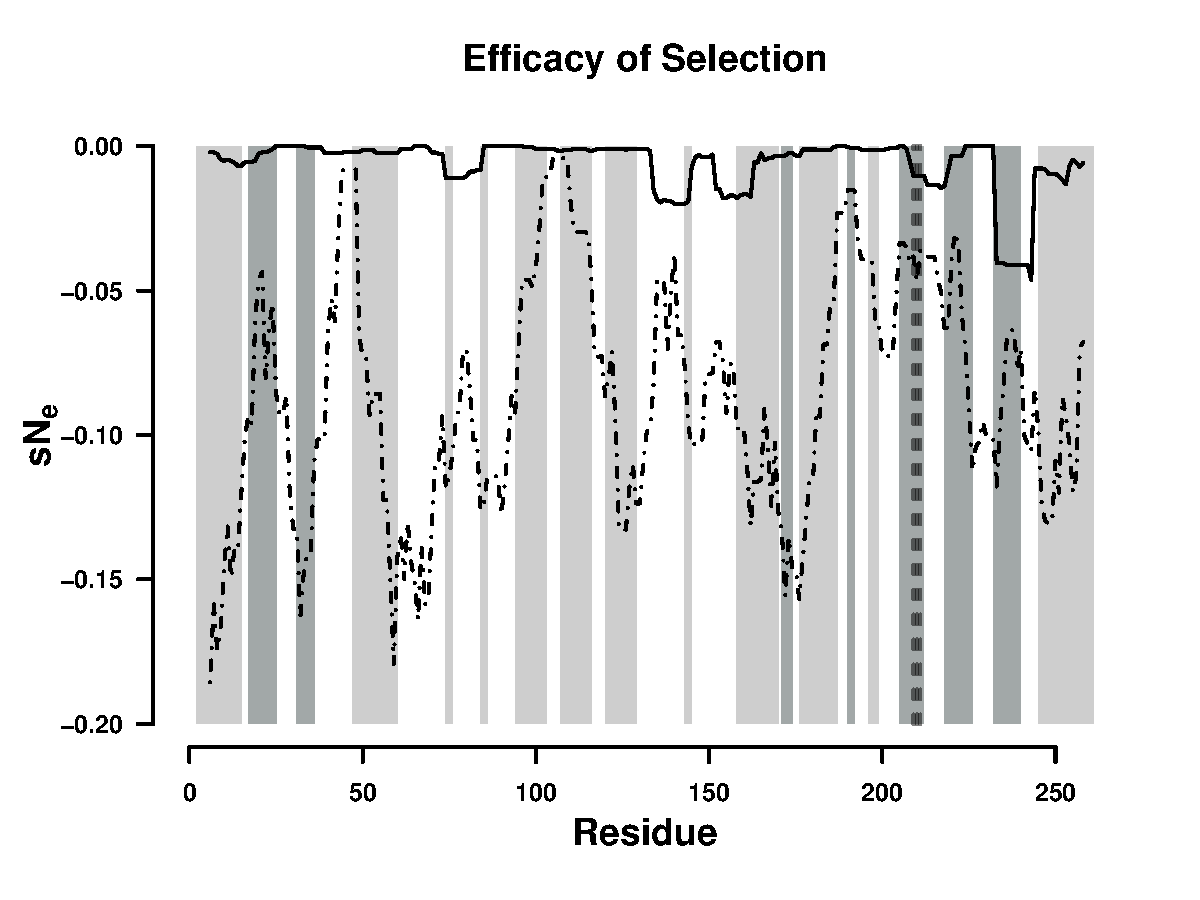
\includegraphics[width=\textwidth]{img/sNe_slide_TEM2016}
	\caption{TEM, bars are different seconday structure elements. Dashed dotted line is DMS, solid is SelAC sNe, all lines are means of all sequences, sliding window of 10 sites. vertical lines are active/binding sites.}
	\label{fig:tem2016_sse}
\end{figure}

\begin{figure}[h]
    \centering
    \begin{subfigure}
        \centering
        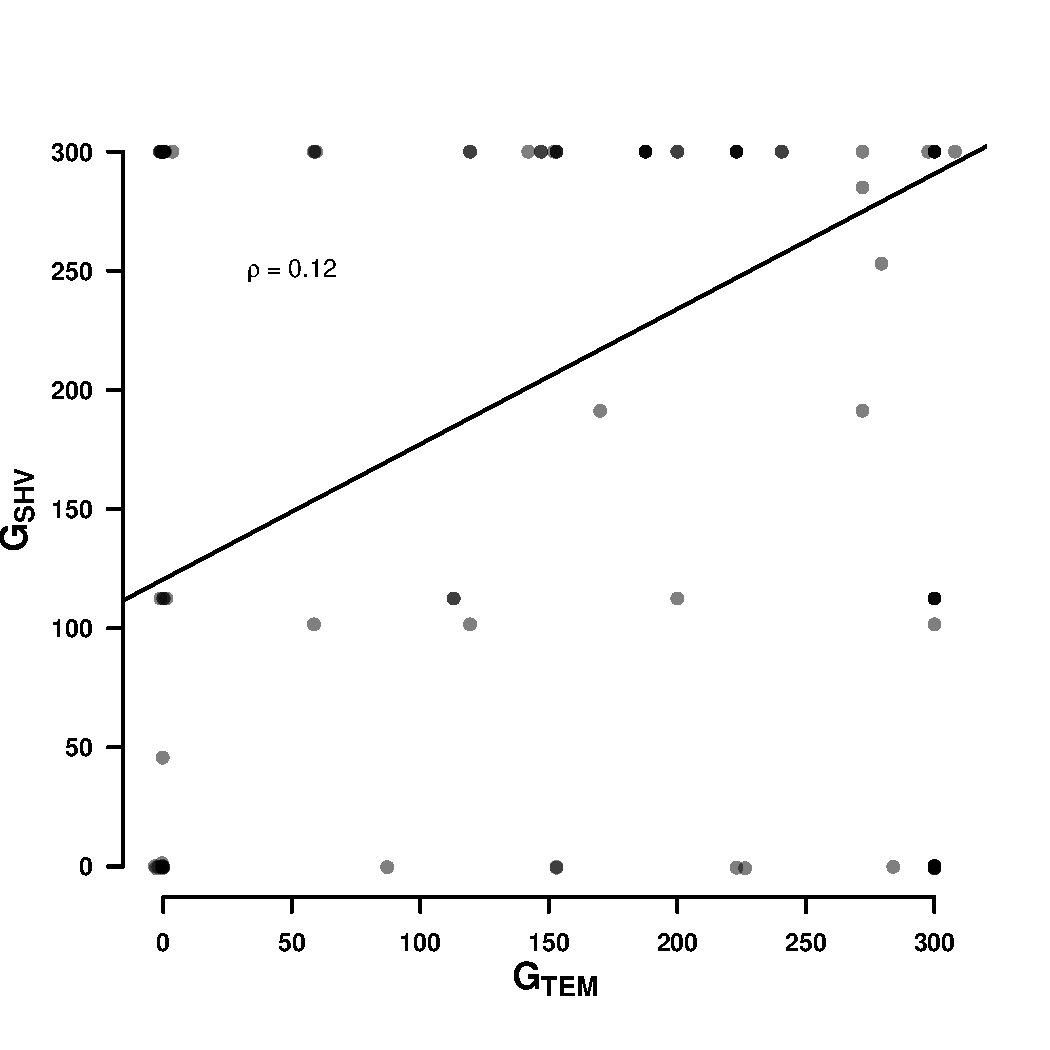
\includegraphics[width=.45\textwidth]{img/g_shift_lac.pdf}
    \end{subfigure}
    \begin{subfigure}
        \centering
        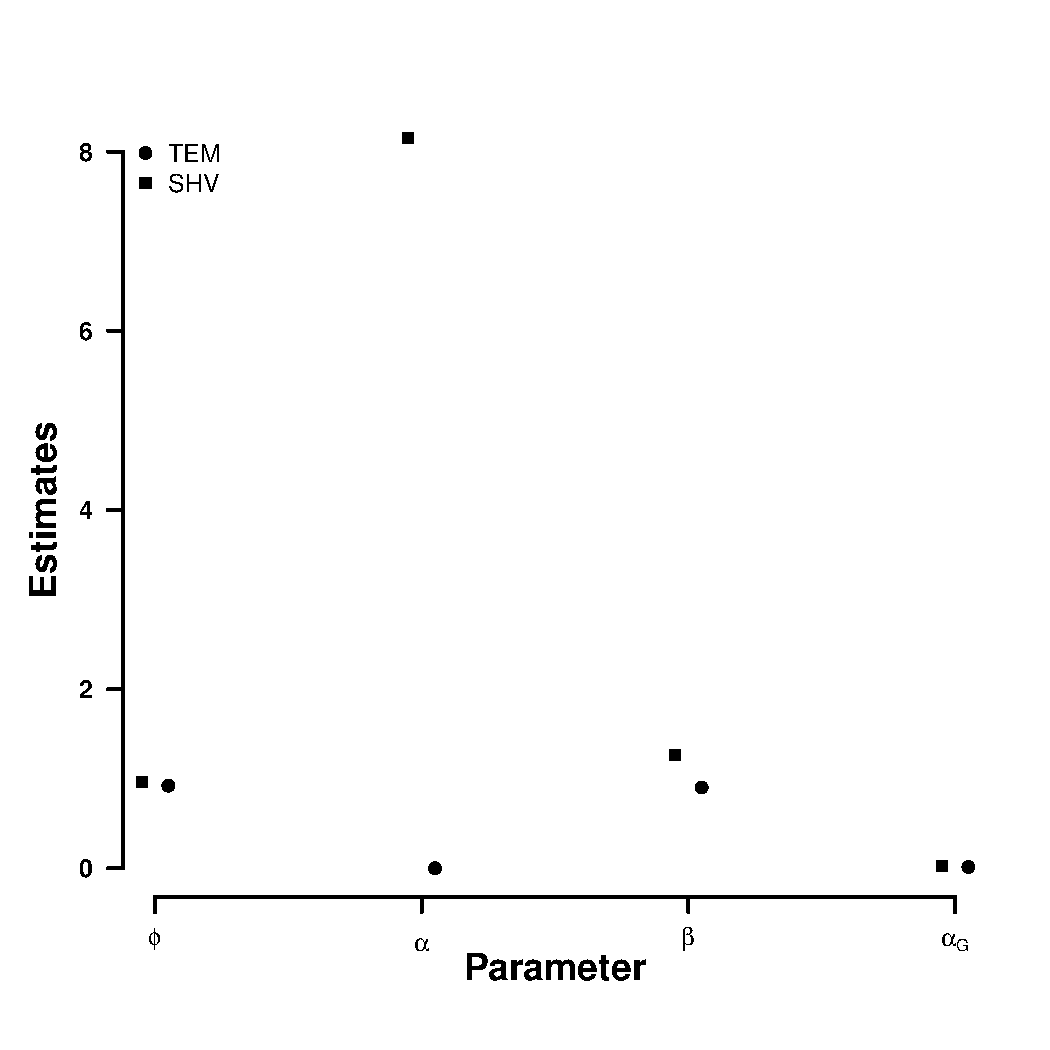
\includegraphics[width=.45\textwidth]{img/TEM_SHV_2016_par_comp.pdf}
    \end{subfigure}
    \caption{Comparisson of selection related parameters between TEM and SHV.}
    \label{fig:tem_shv_param_comp}
\end{figure}


\beginsupplement
\section*{Supplementary Figures}

\begin{figure}[H]
     \centering
	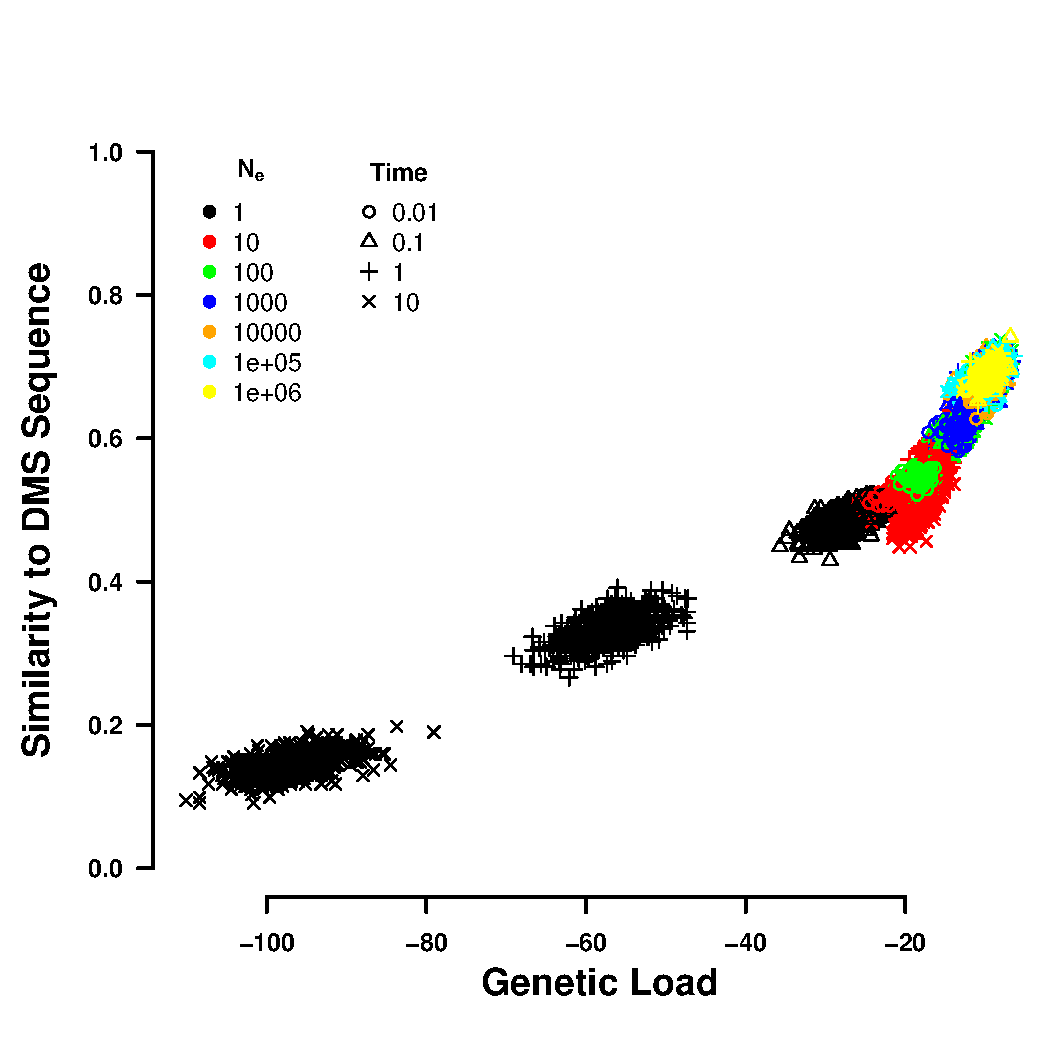
\includegraphics[width=0.6\textwidth]{img/simulated_seqs_gl_dist.pdf}
	\caption{Suppl: Sequences simulated under various values of $N_e$ and for various times. TODO: replace clouds by mean+sd bars}
	\label{fig:sim_seqs}
\end{figure}


\begin{figure}[H]
     \centering
	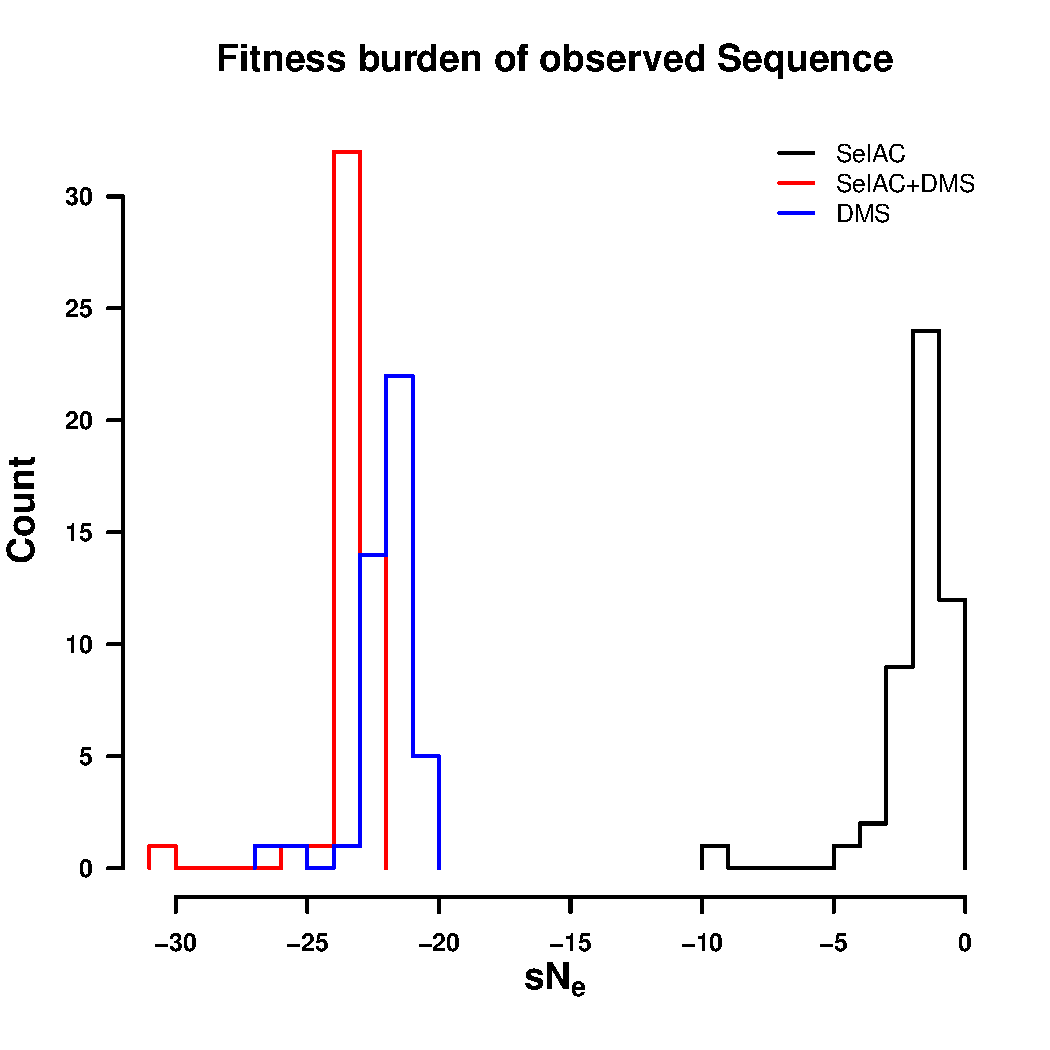
\includegraphics[width=0.6\textwidth]{img/sNe_TEM2016.pdf}
	\caption{Suppl: $sN_e$ of whole sequence, variation across tips. TEM}
	\label{fig:gl_TEM}
\end{figure}

\end{document}
